\section{Fault Tolerance in Specific Space Missions}
\subsection{Voyager Missions}

Voyager 1 and 2 \cite{vo1-nasa}\cite{vo2-nasa} are 2 NASA missions created in
order to explore the outer Solar System
\footnote{http://science.nasa.gov/planetary-science/focus-areas/outer-solar-system/}
The missions were possible due to a rare planetary alignment. Voyager 2 targeted
Jupiter, Saturn, Uranus and Neptune, while Voyager 1 targeted Jupiter and
Saturn. After visiting these planets, they both continued on to chart the far
edges of our Solar System.

There are quite a few works which take a closer look at the Voyager missions.
These missions have brought humanity an unimaginable boost of knowledge about
our Solar System and even beyond. R. L. Heacock presents, in one of his
papers~\cite{tvs}, various engineering aspects of the two spacecrafts.

The two spacecrafts have been launched into space on 20th of August,
respectively 5th of September in 1977. Their trajectories were controlled
through the use of the gravity field and orbital velocity of the planets. This
was the key factor which allowed the encounter with multiple planets. The way in
which the planets where aligned at that time has allowed for each spacecraft to
pass by more planets and it has also helped by reducing the time needed to reach
these planets (e.g. from 30 years normally for a flight to Neptune, the travel
time was reduced to only 12 years).

Before the mission started, hundreds of computer simulations for the
trajectories were carried out. Also, to assure fault protection, research was
made in order to design a self test and repair (STAR) system for the
spacecrafts, as well as an on-board computer access telemetry system (CATS). The
latter allowed STAR to monitor the on-board performances or failures of the
spaceship and, in case it would be needed, to take measures for remedying the
problem.

The spacecrafts had special needs that defined parts of their appearance.
For example, Voyager needed a large diameter antenna since the communication
needed to be possible despite the very long distance to Earth. It also had an
external surface which needed to be adequate for the temperatures and radiation
it was facing. Internally generated heat was enclosed with the help of special
blankets which were insulating. Also, most of the subsystems had replacement
heaters.

The attitude control system (ACS) was used in order to keep the antenna in the
right position needed for communication. The ACS was also in charge of keeping
or modifying the spacecraft's trajectory. A block diagram of the ACS can be seen
in Figure~\ref{fig:voyager_bd}.

\begin{figure}[htb]
	\begin{center}
	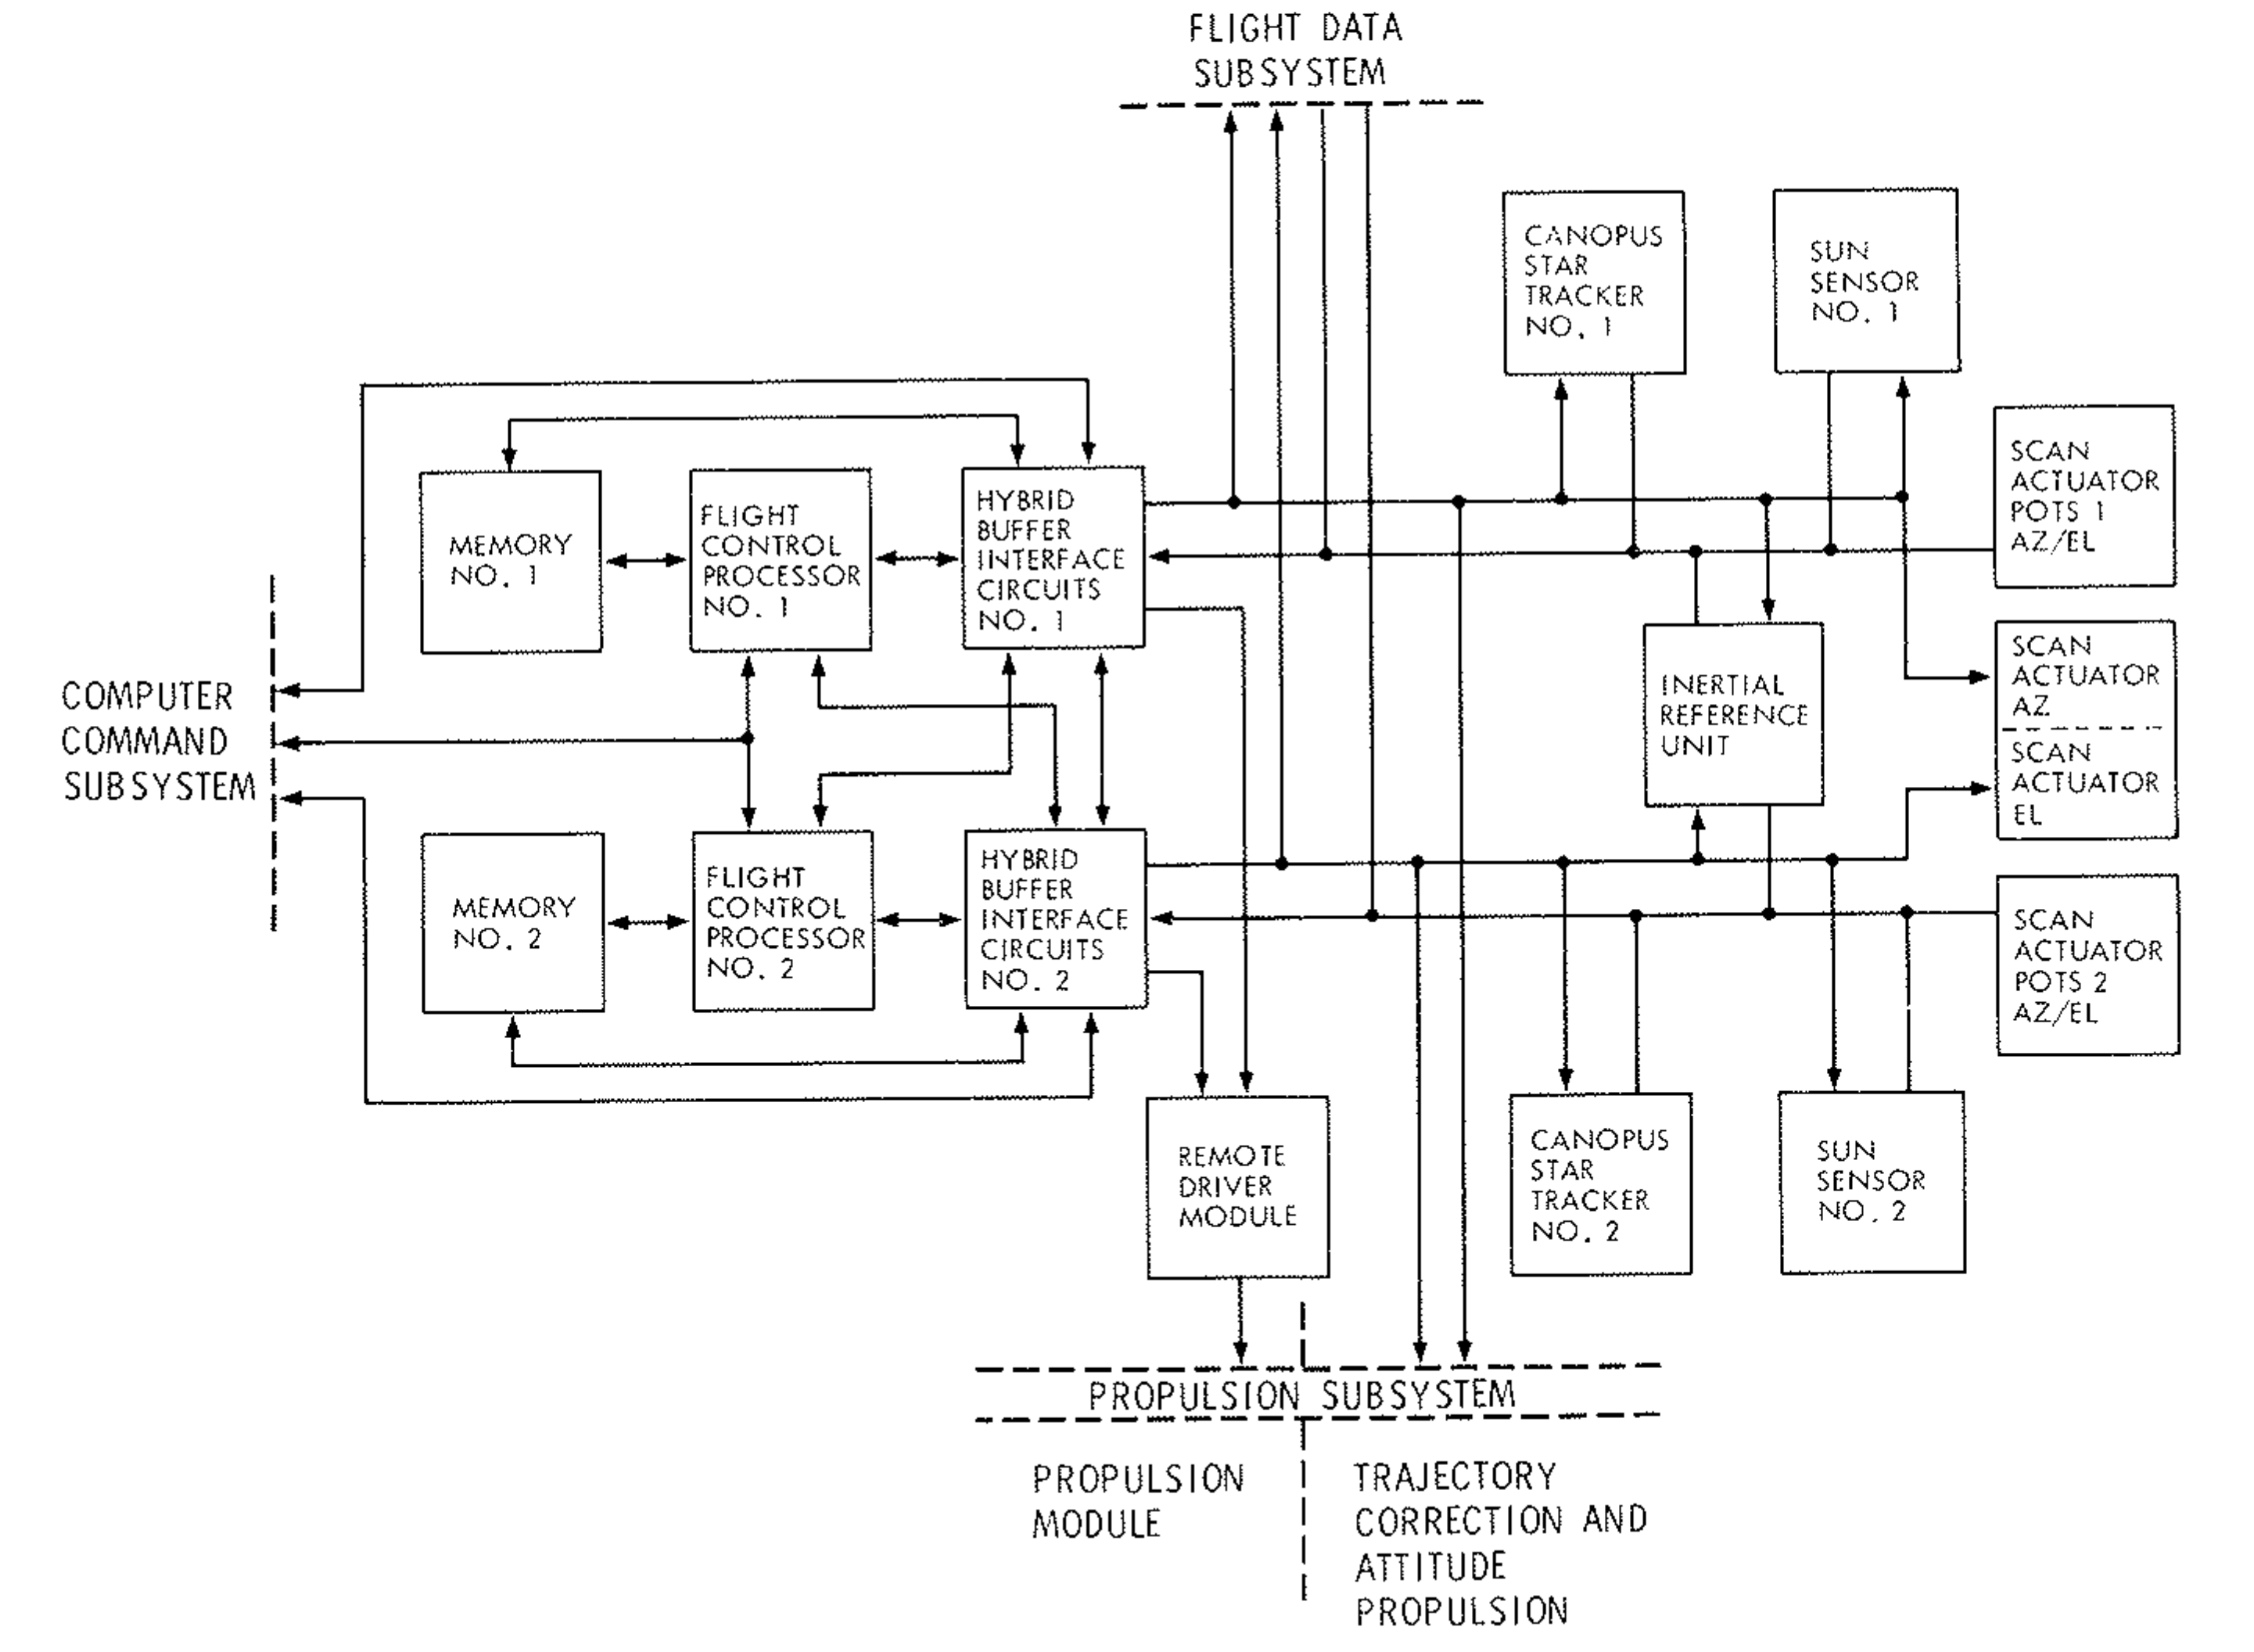
\includegraphics[width=0.92\textwidth]{img/voyagerACS.png}
	\caption{The block diagram of Attitude Control Subsystem on
	Voyager. \small{\textit{ Source: R.L. Heacock, The Voyager Spacecraft, 1980}}}
	\label{fig:voyager_bd}
	\end{center}
\end{figure}

The spacecrafts kept track of their position by using the Sun and a star
(Canopus). The sensors that keep track of both the Sun and Canopus are block
redundant in order to ensure that the spacecrafts will be able to compute their
position and that complete failure in doing so would be unlikely. There is,
additionally, a periodic calibration of the Sun sensor. This allows keeping the
accuracy level needed in order for the spacecraft to position the scan platform
so that it accurately points the remote sensing instruments. In case the sensor
that keeps track of the Sun position is not working and the solar panels cannot
be pointed in the right direction, the spacecraft has an inbuilt solar
independent power system given by the radio-isotope thermo-electric generators.
This ensures that even if the spacecraft cannot use the Sun as a power supply,
it can still maintain functionality. 

Great amount of testing was also done in order to ensure that, in case of an
accident at launch time, the radioactive material which existed on board the
spacecraft would be contained and would not represent any danger. This is
possible because the shells that contain the plutonium spheres were wrapped in
an impregnated graphite yarn which provided a good energy absorption in the case
of an accident.

Since in the later stages of the mission, the spacecraft needed to wait for
almost three hours for a response from the ground base, it was obvious from the
beginning that it would need to have at least some operations done autonomously.
However, control parameters and even control laws could be re-programmed in
flight in case it is necessary. This has allowed solving several in-flight
problems that have occurred throughout the years~\cite{litty} simply by sending
software patches.

The computer and control subsystem fault correction and detection routines
incorporate internal error and power levels checks, received command and
transmitted signal loss, spacecrafts maneuver faults, attitude control subsystem
failures and many others. For example, the command loss routine verifies if any
commands have been given to the spaceship. A timer is used in order to make
checks to see if commands have reached the spaceship components or not. If a
command has been given and received, then the timer is reset. In case the
command is either not received or was not given when expected, the command loss
routine stars, meaning that a series of re-configurations are initiated.

A description of the error detection mechanism for the attitude control subsystem
is given in~\cite{ft-space-avionics}. It consists of:
\begin{itemize}
  \item failure of receiving a 'I am healthy' report every 2 seconds by the
  command control subsystem
  \item loss of references to Canopus or the Sun
  \item failure of re-writing memory every 10 hours
  \item taking more time to adjust trajectory than expected
  \item gyro failure
  \item power supply failure
  \item parity error on commands received from the command and control subsystem
  \item unresponsiveness to commands
  \item incorrect sequence of commands
\end{itemize}

A high redundancy of subsystems and hardware was used when designing the two
spacecrafts. This has proven to be a good safety measure since, for example,
the receiver for Voyager 2 has malfunctioned and almost could have caused the
failure of the mission. However, the problem has been identified fast and the
spacecraft has been functioning on the back-up receiver since 1978. The attitude
control subsystem is made of redundant computers (one of them is a standby which
is ready to take the other's place if needed). The command and control subsystem
also has redundancy incorporated in it. However, in this case, the redundant
computer monitors the functional computer.

Voyager 1 and 2 have achieved their goals and have surpassed them. They have
made unexpected discoveries (e.g. at least nine active volcanoes on
Io\footnote{Io is one of the Jupiter moons}~\cite{tvs}) and are currently the
most distant human made objects. Voyager 1 has already left our solar system in
2012\footnote{http://www.space.com/22729-voyager-1-spacecraft-interstellar-space.html}
and is currently traveling through interstellar space.

\subsection{Cassini-Huygens}

The Cassini-Huygens~\cite{ch-nasa} mission was a NASA-ESA joint mission aimed to
study Saturn, its moons and its rings. The two names that form the name of the
spacecraft are present because Cassini represents the NASA-supplied spacecraft
while Huygens represents the lander designed by the European Space Agency.
Cassini was the first spacecraft to actually orbit Saturn~\cite{ch-nasa}.

An interesting description of the fault tolerant design of both the Cassini
spacecraft and the Huygens probe is given in D.P Siewiorek and P.
Narasimhan's article~\cite{ft-space-avionics}. The Cassini orbiter was also
developed with possibility of self-recovery in mind, since it would take awhile
before any answer could be transmitted back from Earth.

The Huygens probe~\cite{hygens} has landed on Titan on 14th January 2005. It's
purpose was to make a variety of measurements. It was formed out of various
subsystems. Among them we can find the ones that are in charge of overseeing the
mechanical and thermal components, probe-relay data, command and data management
and electrical power. The states of each of its subsystems are influenced by the
mode in which the probe is at a particular moment of the mission. The modes it
can enter are: cruise, coast, entry and decent. Huygens' mission aimed to last
for the 2.5 hours it took for it to descend in the atmosphere of Titan.

The Huygens' fault tolerant design was focused on autonomy. This was needed
because the probe could not have been commanded after its detach from the
spacecraft, due to distance from Earth. The probe had a completely redundant
electrical architecture (most specifically it used block redundancy) and the
software architecture also used redundancy. It also had two identical command
and data management units, a triply redundant mission timer unit as well as a
triply redundant central acceleration sensor unit. Huygens also had double
redundant accelerometers and double redundant proximity sensors.

The 2 identical command and data management units have been developed with only
small differences that aimed to avoid common-mode failures. They both execute
their own software as to be able to run on their own, if needed, in order to
keep the mission afloat. Also, a delay was introduced so that, in case there
would be a problem generated by the temporarily loss of the telemetry link, a
fault could be avoided since the two replicas had a delay between their telemetry
of 6 seconds. Both of the two units do checks and consider themselves invalid in
the case they discover that they have a two bit error in the same word in the
memory or an under-voltage value of the power line.

In order to ensure that the experimental results and collected data were safe,
Huygens probe was not the only sending them to Earth. They were, in fact, also
kept as a copy in the Cassini orbiter so that, in any case, they could be
transmitted to the ground team on Earth.

Cassini's fault protection mechanisms~\cite{cassini} aimed to avoid the
possibility of having a single point of failure somewhere in the systems which
formed the orbiter. Other goals the fault protection mechanisms had where to
make possible the system recovery and reconfiguration from multiple faults, in
case these faults would take place in regions which were independent.

The approach the Cassini system fault protection used was that it was driven by
the priority of the faults identified and it could work on the recovery of only
one fault at the time. More faults could have the same priority assigned to
them, but they would be served in a first come first served manner. The way in
which priority was assigned to faults is that the ones which would take the most
to be solved would be assigned a lower priority while the most time-critical
ones would have the highest priority~\cite{ft-space-avionics}.

The primary mission of the Cassini orbiter ended on 30 June 2008. It did achieve
all the original goals and then moved on to take on a new mission - to observe
and gather data about the seasonal changes brought by the Sun's changing angle
on Saturn. It has also continued to study the rings and moons of Saturn, sending
back to Earth priceless information and knowledge about the seventh planet from
the Sun~\cite{ch-nasa}.

\subsection{Mars Climate Orbiter}
Mars Climate Orbiter (MCO)\cite{mco-nasa} was part of the NASA Mars Surveyor
program which included the Mars Global Surveyor as well as Mars Polar Lander. It
was launched in 1998 with the main objective of studying the climate of Mars. It
aimed to monitor atmospheric dust and water vapor as well as taking pictures of
the planet's surface in order to gain insight on the climatic changes. The hope
was to gather evidences that would support the theory of existing water
underneath the surface of the planet.

MCO was also designed to serve as a communication relay for the Mars Polar
Lander, however after the Lander's mission, it was supposed to conduct its own
main mission independently.

After its nine months journey to Mars, MCO was lost because it missed its planned
orbit altitude and fell into the Martian atmosphere where it was destroyed.

The problem identified in the NASA Mishap Investigation Board Phase I
Report~\cite{mco-rep} was that the MCO failed to use metric units in the coding
of a ground software file used in trajectory models. Other causes that
contributed to the failure of the mission included system engineering, training
and organizational factors.

In order to understand better the circumstances that lead to the failure of this
mission, we need to take a closer look at the Attitude Control System and the
fault protection architecture of the MCO~\cite{surv-nasa-mars}.

The MCO's Attitude Control System contained a Sun sensor, an inertial
measurement unit, a star camera and reaction wheels. The MCO was controllable in
roll, pitch and yaw so that it could adjust its altitude, perform trajectory
maneuvers and achieve Mars Orbit Insertion. It was designed so that it could use
the gravity force of Mars in order to adjust to the needed velocity which could
allow it to keep the desired orbit and altitude. The design included rocket
engine modules which allowed this as well as serving as elements that dissipated
any angular momentum which could be accumulated in the reaction wheels. The
Spacecraft Performance Analysis Software (SPAS) was used to calculate the
angular momentum desaturation, however it was not using the correct units of
measure (error in the Newton to lb-f conversion). This has lead to MCO
estimating badly its altitude and orbit and thus, its failure to maintain
orbit.

The fault protection capabilities were unsatisfying at a number of levels in
this mission. First of all, there was an error in the human management process.
The calculation of the automatic momentum desaturation involved a human
constant, because people where involved in loading the information to servers,
also in retrieving it from servers and up-linking it to the MCO. The teams
dealing with the information where not specifically the ones who introduced the
error, however they could have observed the problem and could have found a
solution to solve it. This proves the existence of a fault in the human-system
interaction. This could have been avoided by developing a better system that
would allow people to assess the correctness of the output data based on the
input they are giving. It could be a software solution that would act either as
verifier (just calculate and report the expected results) or as a checker that
would identify the inconsistency and report it.

The critical problem in the MCO case was the lack of an adequate converter
between the Newtons and lb-f. The software used for the MCO was partly carried
over from another mission (The Mars Global Surveyor). The previous mission used
a converter, however it was not imported for the MCO mission by mistake. The
fault could have been avoided if there would have been thorough testing after
the importing of the already existing software. If the re-used functions would
have been inspected with attention and tests would have been developed in order
to check the correct functionality in the new context, the fault could have been
discovered and solved.

The expectation to have a software system with no bugs or problems is quite
unrealistic. However this should not affect the success of missions. The MCO was
already calculating the angular momentum desaturation and afterwards
down-linked it to the ground base. At that point the Spacecraft Performance
Analysis Software was used in order to calculate the angular momentum
desaturation value without making the correct conversion between Newtons and
lb-f. However, the result would be provided to the team in charge and only
afterwards the plan for the future actions would be up-linked to the spacecraft.
In this case, another solution for fault avoidance would have been the
limitation or elimination of the need of the spacecraft to rely on external
systems and human intervention. Basically, if the MCO would have been designed
to be able to calculate its own position and only then cross check it with the
available data provided by the ground team, it would have been possible to at
least notice and report the problem.

In order to have a good failure tolerance, it was decided that for future
spacecrafts it would be advised to use redundant and independent components
(both software and hardware). In the case of performing the same calculations
with the use of various software modules it could be possible to identify the
differences in the values. In the case of multiple such components, a voting
could be implemented in order to rule out the modules that provide wrong
results.

Since this case is mainly a failure caused by the inadequate re-use of software,
it can be stated that such errors can be avoided through the use of independent
evaluation and validation of the re-used software. The use of regression
testing~\footnote{http://en.wikipedia.org/wiki/Regression\_testing} as well
as comparing results to expected outputs can prove helpful.

\subsection{Mars Reconnaissance Orbiter}

The Mars Reconnaissance Orbiter (MRO)\cite{mro-nasa} was launched on the 12th of
August, 2005 and it was one of the first spacecrafts entering Mars' orbit.

Its journey to Mars lasted seven months and it took six more months afterwards
in order for it to reach its science orbit. The MRO was created with the purpose
of tracking changes of the water and dust in Mars' atmosphere. It was also
supposed to look for more evidence of ancient seas and hot springs and to study
the climate changes based on Mars' surface minerals. It also serves as a data
relay station for other missions.

The objectives of the MRO where complex and the probability of failure was high
because of this. There were multiple things that could go wrong with the
mission, considering the complexity of its overall goals and functionality
expectations \cite{tvs}.

First of all, the mission was supposed to last about 5.4 years. The system on
the spacecraft was supposed to have an up-time as close as possible to 100\%
during this mission. This is hard to achieve because all possible failures need
to be prevented or handled without losing functionality or precious data.

An analysis of the fault pretection architecture, the effectiveness of this
architecture as well as a categorization of the fault protection capabilities of
the MRO are described in detail in \cite{surv-nasa-mars}.

In order to assure that no big failures cand occur and that, despite its
complexity, the system will work accordingly in order to achieve the mission's
goals, a semi-autonomuos fault protection software (SPIDER - SPacecraft Imbedded
Distributed Error Response) has been developed for the MRO. It has been
developed in C-language with the possibility of re-use for any other future
missions. SPIDER can support redundancy and cross strapping tasks, requirements
which the MRO is supposed to meet.

Despite it's advanced capabilities and the fact that it acts as a first
responder to erros and handles most of them, SPIDER was not design to function
on its own. It still needed help from the ground in order for the system to be
set back in a normal state for the cases when it entered a safe mode. Also,
ground operations where needed in case the system did not recognise some
possibly threatening conditions that could appear. The main advantage of the
SPIDER is that it can actually prevent the system from entering massive failure
without the need to wait for the ground crew to notice and react to the
problems. The decission process of the SPIDER can be seen in
Fig.~\ref{fig:spider}.

\begin{figure}[htb]
	\begin{center}
	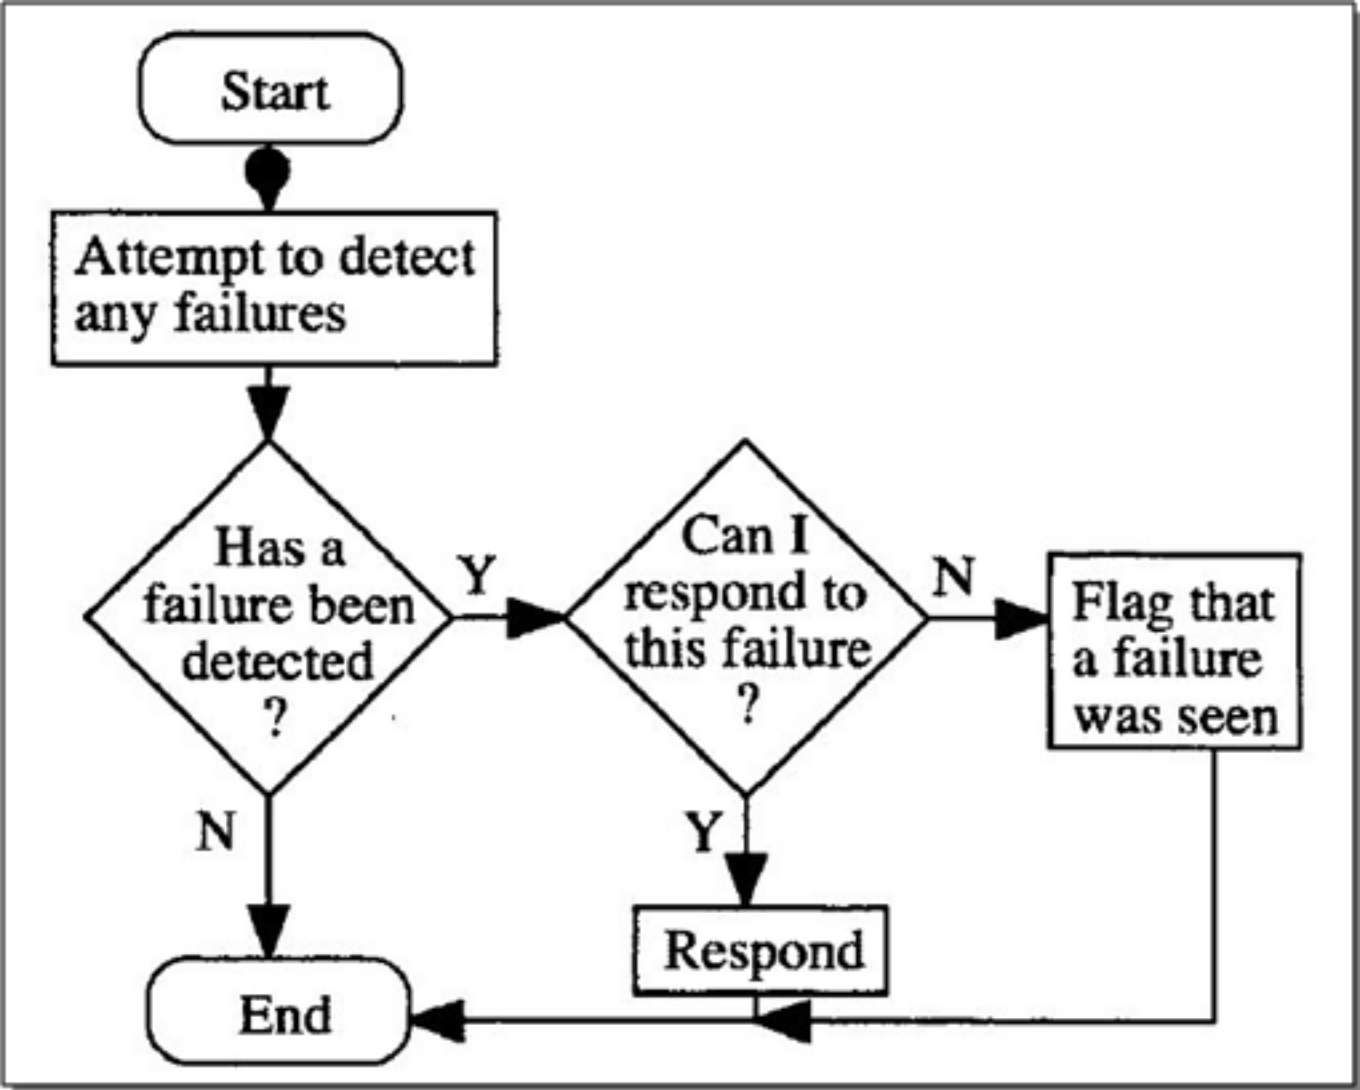
\includegraphics[width=0.5\textwidth]{img/spider.png}
	\caption{The generic decission process of the SPIDER\small{\textit{ Source: E.
	Scale, The evolution of a spider fault protection, incremental development, and
	the mars reconnaissance orbiter mission, 2003}}}
	\label{fig:spider}
	\end{center}
\end{figure}


The SPIDER ensures that the fault responses are general. For example, if the MRO
finds itself in a position in which a fault is detected, then it automatically
switches to a safe mode and interrupts all the uncritical equipment and
functionality. The system can be turned back to normal functionality from the
ground level by the team in charge after following a defined protocol.

The SPIDER ensures that the MRO is not affected by fails at any given time, with
the presumption that only one system can generate failure at a given time. It
basically tries to ensure that the MRO is completely single-fault tolerant and
this leads to the robustness and high relability level of the architecture. As
it was mentioned before, SPIDER was created around the idea of keeping things
redundant and around the cross strapping concept. Among the
redundancy technics it uses we can identify: block redundancy, functional
redundancy, cooperative redundancy and cross strapping.

The architechture of the SPIDER is hierarhical. It has three software
levels: the component level fault protection which is used for communication
with the MRO hardware, the performance level fault protection which keeps track of the
performance of each subsystem and the system level fault protection which tries
to keep failures from happening. Depending on the type of failure, it can be
handled by the befitting logic. In order to avoid starvation, the higher levels
in the hierarchy are allowed to call on to the lower levels in order to assign
them specific tasks, but they cannot take priority of the tasks which
already are executing in these levels.

The SPIDER has been thorughly tested before being integrated on the MRO, but a
final proof of its capability was the fact that, even though the MRO has
encountered quite a few failures during the mission (e.g. memory corruption,
downlink connectivity failure, etc.), it was capable to recover and to achieve
the mission's goals.

\subsection{Mars Exploration Rovers}

NASA has launched in 2003 the twin rovers, Opportunity and Spirit
\cite{mer-nasa}, with the purpose of gaining more insight about past water
activity on the red planet and if there where, at some point, conditions that
could favor life on our neighbor planet. The planned mission was supposed to
last for about 3 months from the moment the rovers would land. However, they
have exceeded any expectations both as far as their durability is concerned as
well as the discoveries they have made.

Spirit has collected evidences that, in the past, Mars was much wetter than we
see it know. Also, it collected information about the wind on the red planet.
The rover has been silent as of March 2010 and the ground team has ceased to try
to contact it since May 2011 when its mission was closed and considered
complete.

Opportunity has found evidence that Mars could have been capable of sustaining
microbial life. During its mission it traveled for over 20 km (as of March 2010)
in its search for a better understanding of the planet. The rover is still
active (as of 5th November 2013).

An overview of why the fault protection worked so well for these rovers is
provided in \cite{surv-nasa-mars}.

The rovers needed to enter into a sleep mode during the days in order for them
to be able to recharge their batteries. In this state their CPU would be powered
off, but the hardware still needed to maintain the safe thermal and power states
(the temperatures on Mars can be quite extreme - from negative
107$\,^{\circ}\mathrm{C}$ up to over positive
30$\,^{\circ}\mathrm{C}$\footnote{http://en.wikipedia.org/wiki/Climate\_of\_Mars}).

Upon waking from the sleep mode, the rovers were expected to start the
communication without any help from ground operation teams on Earth. As a fault
protection measure, if during the rover's initialization a server error occured,
the reset of the system would be postponed for a pre-defined amount of time. A
software health function was also used in order to check for any lingering or
suspended tasks. For the communication system, redundancy was used such that, in
case the high gain antenna would not function properly, then the low gain
antenna would perform its tasks (even if this one had lower data rates it could
still be enough so that the mission wouldn't be a failure).

The surface fault protection architecture of the rovers can be divided into
local and system level fault protection, each of them dealing with various kinds of
problems. The local and system level fault protection can be seen in detail in
Fig~\ref{fig:rovers}.
\cite{fprot}
\todo{Care e faza cu zona asta? - solved? citeste acum}

\begin{figure}[htb]
	\begin{center}
	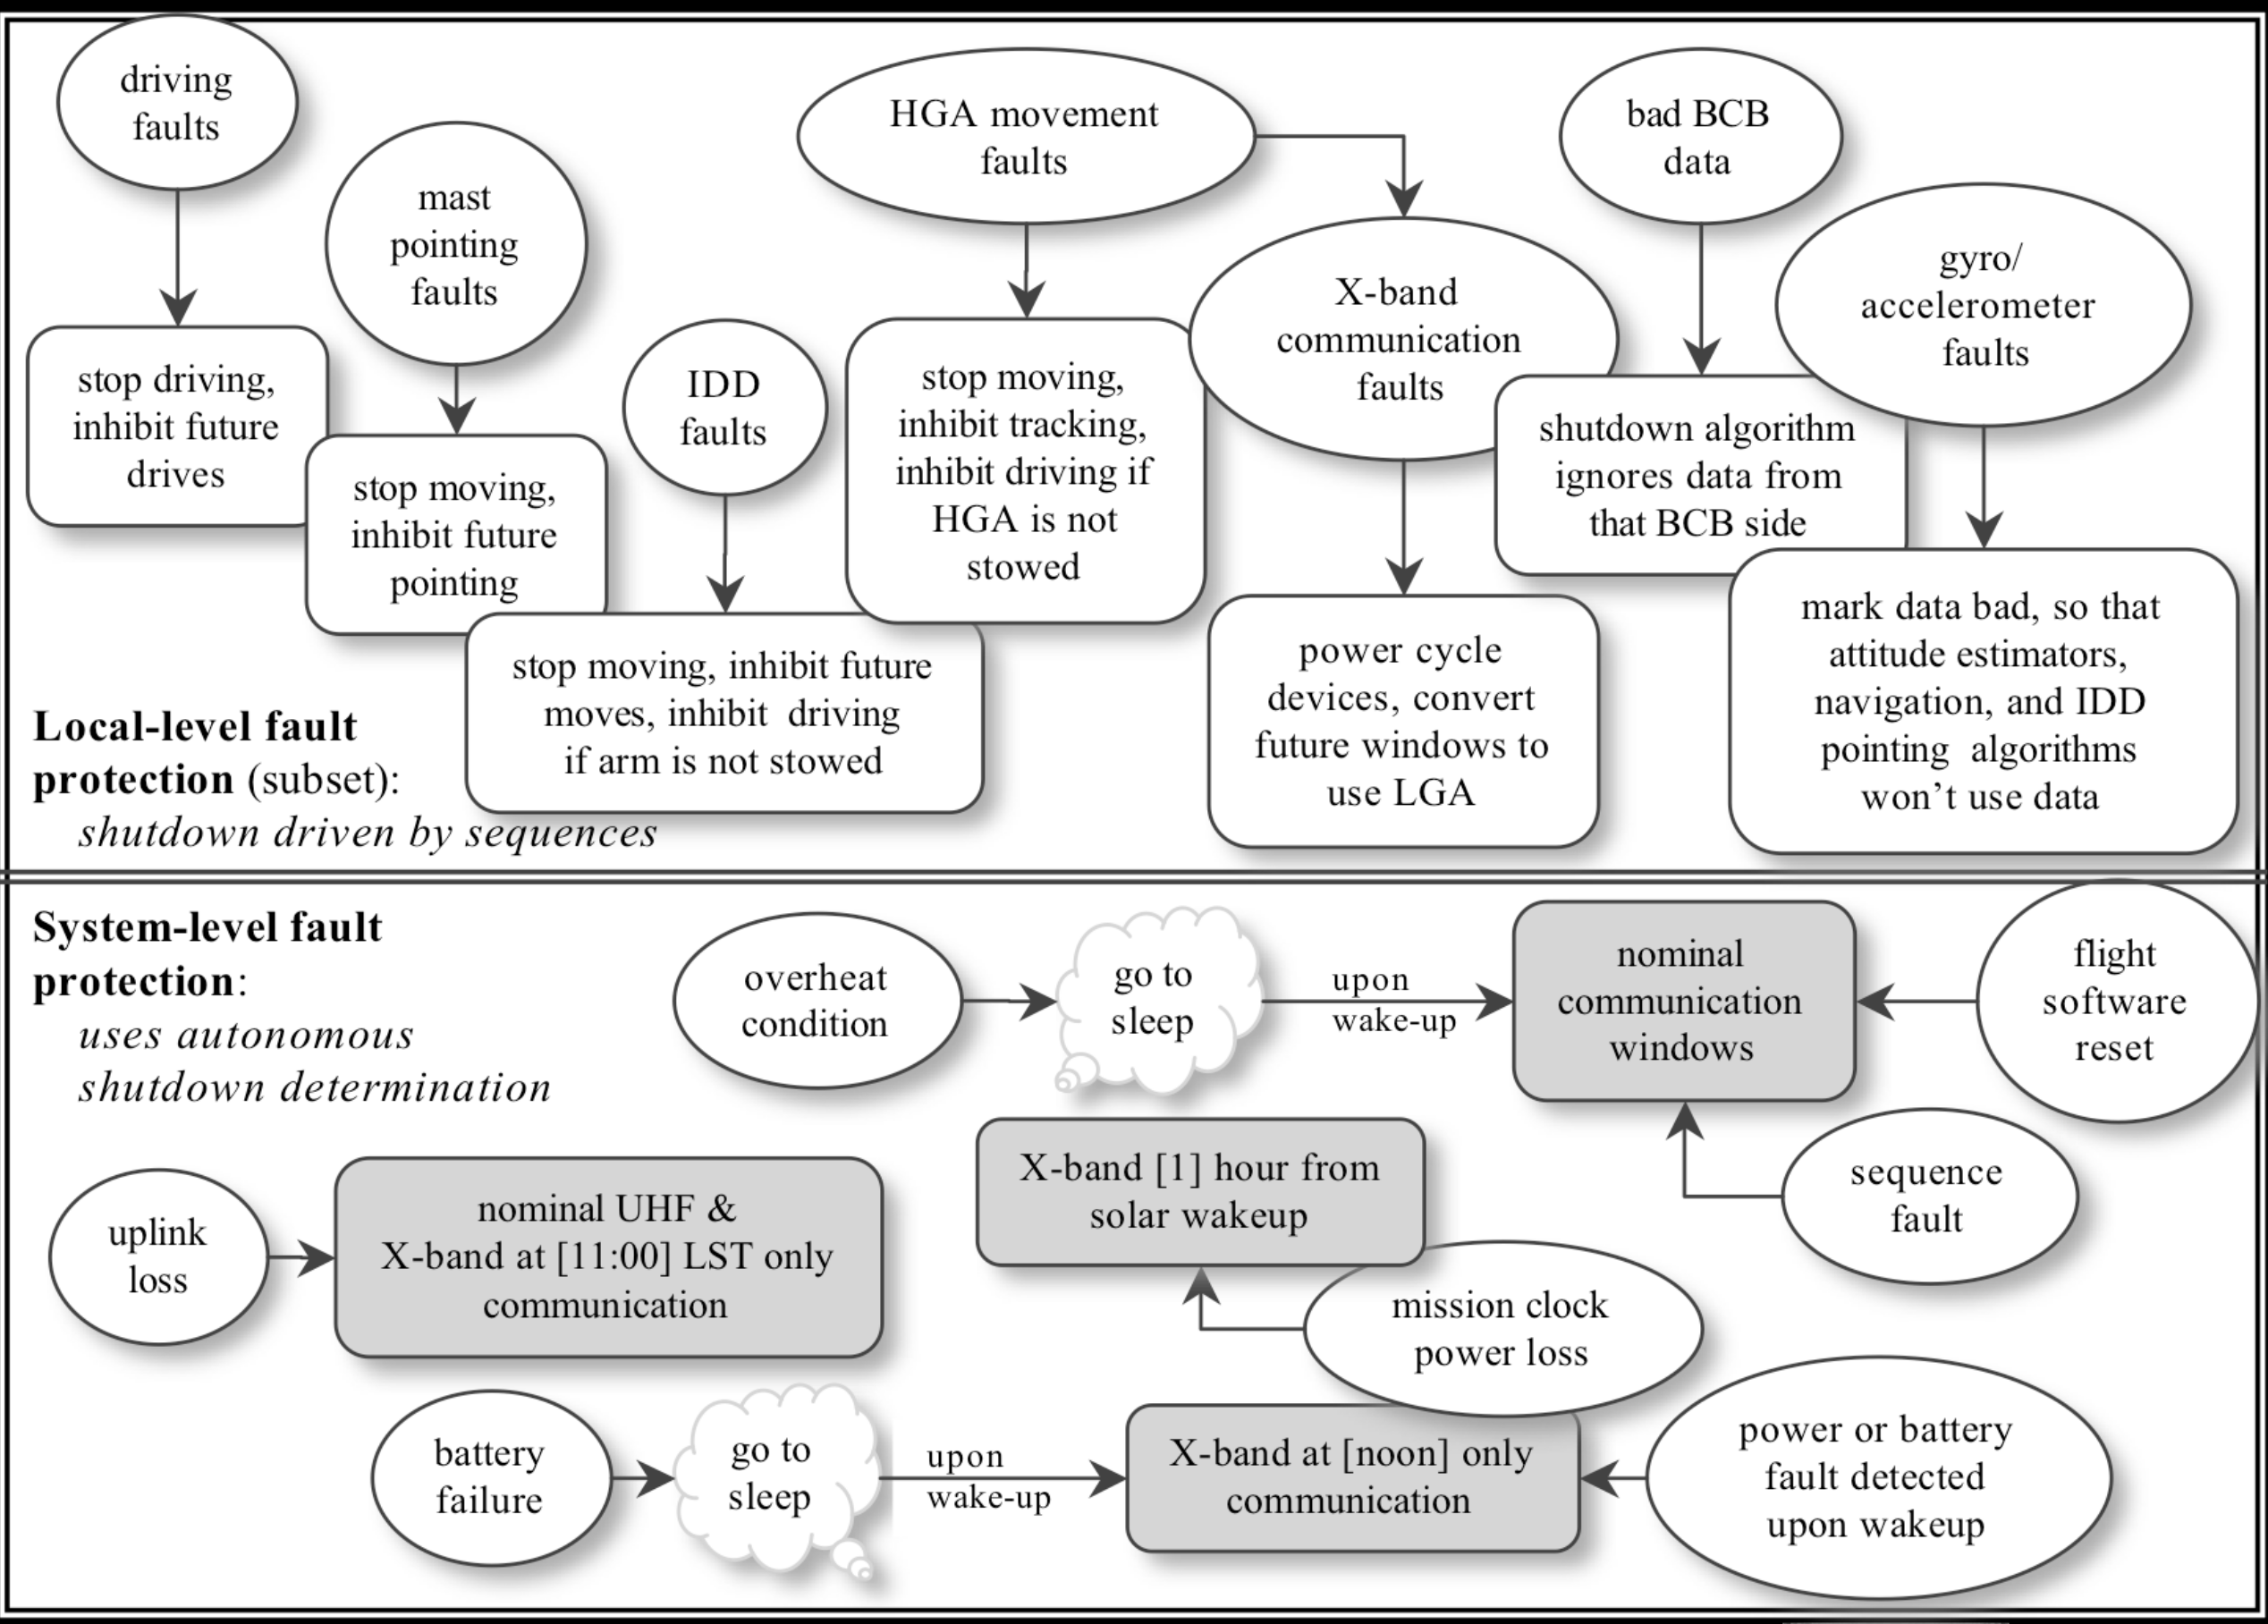
\includegraphics[width=0.92\textwidth]{img/rovers.png}
	\caption{Attitude Rovers surface fault protection\small{\textit{ Source: D.
	Clark, C. Brennan and M. Jaunich, Survey of Nasa Mars Exploration Missions -
	Software Fault Protection Architecture, 2010}}}
	\label{fig:rovers}
	\end{center}
\end{figure}

There are more general capabilities of the fault protection architecture used in
the case of the rovers. First of all, the ground teams can monitor the data
which the rovers send back (or fail to send back) and can intervene based on the
type of errors they observe.

Since the rovers have an algorithm that controls automatically the wake up and
shutdown procedures, it means that a low energy fault can be avoided. The
algorithm only allowed the rovers to work when they had enough energy to do
this, thus abnormal terminations or uncapability to save data before entering
sleep mode could be avoided. 

A plus to the fact that the rovers needed to enter sleep mode everyday and
basically shutdown for a period of time was software
rejuvenation\footnote{http://en.wikipedia.org/wiki/Software\_aging}. Memory
leaks could be removed through this process.

The rovers were also tolerant to failure because, for example, in case they did
not stock up enough energy in order to function properly, than the system would
not allow them to wake up from the sleep mode and by doing this it avoided the
failure of letting them work without appropriate power. Aside from this, they
benefited from the presence of a navigation algorithm that looked for possible
hazards on the rovers' paths and tried to avoid them by chosing between posible
identified routes.

Even thogh testing was developed previous to mission launch, complete fault
avoidance could not be guaranteed. The ground team could identify that after 17
sols (Martian days) one of the rovers was rebooting over and over. They managed
to identify the problem as being the fact that when a file needed to be deleted
from RAM, even though the link to it was lost, the size of the table of contents
of the RAM was not decreased so the system managed to consume all the RAM space
available after some time. The problem was solved from the ground when the team
instructed the software to not use the memory and use another one instead. This
prevented the failure of the mission.
